% TODO
%
% - Fotos der Räder und Anordnung
% - Fotos des Roboters
% - Diskussion der Ergebnisse

\documentclass[a4paper]{article}

\usepackage[utf8]{inputenc}
\usepackage[T1]{fontenc}
\usepackage{lmodern}
\usepackage[ngerman]{babel}
\usepackage{amsmath}
\usepackage{nicefrac}
\usepackage{graphicx, wrapfig, float}
\usepackage[onehalfspacing]{setspace}
\usepackage{paralist}  % \begin{compactitem}

\title{Kreisfahrten mit einem Roboter mit Mecanum-Rädern}
\author{Manuel Fehmer \\ Thomas Feldmann \\ Marlene Feldmann \\ Carsten Hussmann}

\begin{document}
\maketitle
\newpage

\section{Einleitung}
Der Mecanum-Roboter ist ein omnidirektionales Fahrzeug. Er kann ohne Lenkung aus jeder Position in eine beliebige Richtung fahren. Grund dafür sind die verwendeten Allseitenräder -- Mecanum-Räder -- auf deren Umlauffläche 15 weitere tonnenförmige Hilfsräder angebracht sind. Zur Steuerung des Roboters ist es notwendig ein mathematisches Modell zur Beschreibung der einzelnen Bewegungen der Räder aufzustellen.

Ziel ist es eine Kreisfahrt auf einem Viertelkreis mit dem Durchmesser 4000 mm auf drei Arten zu realisieren.

\begin{figure}[H]
    \centering
    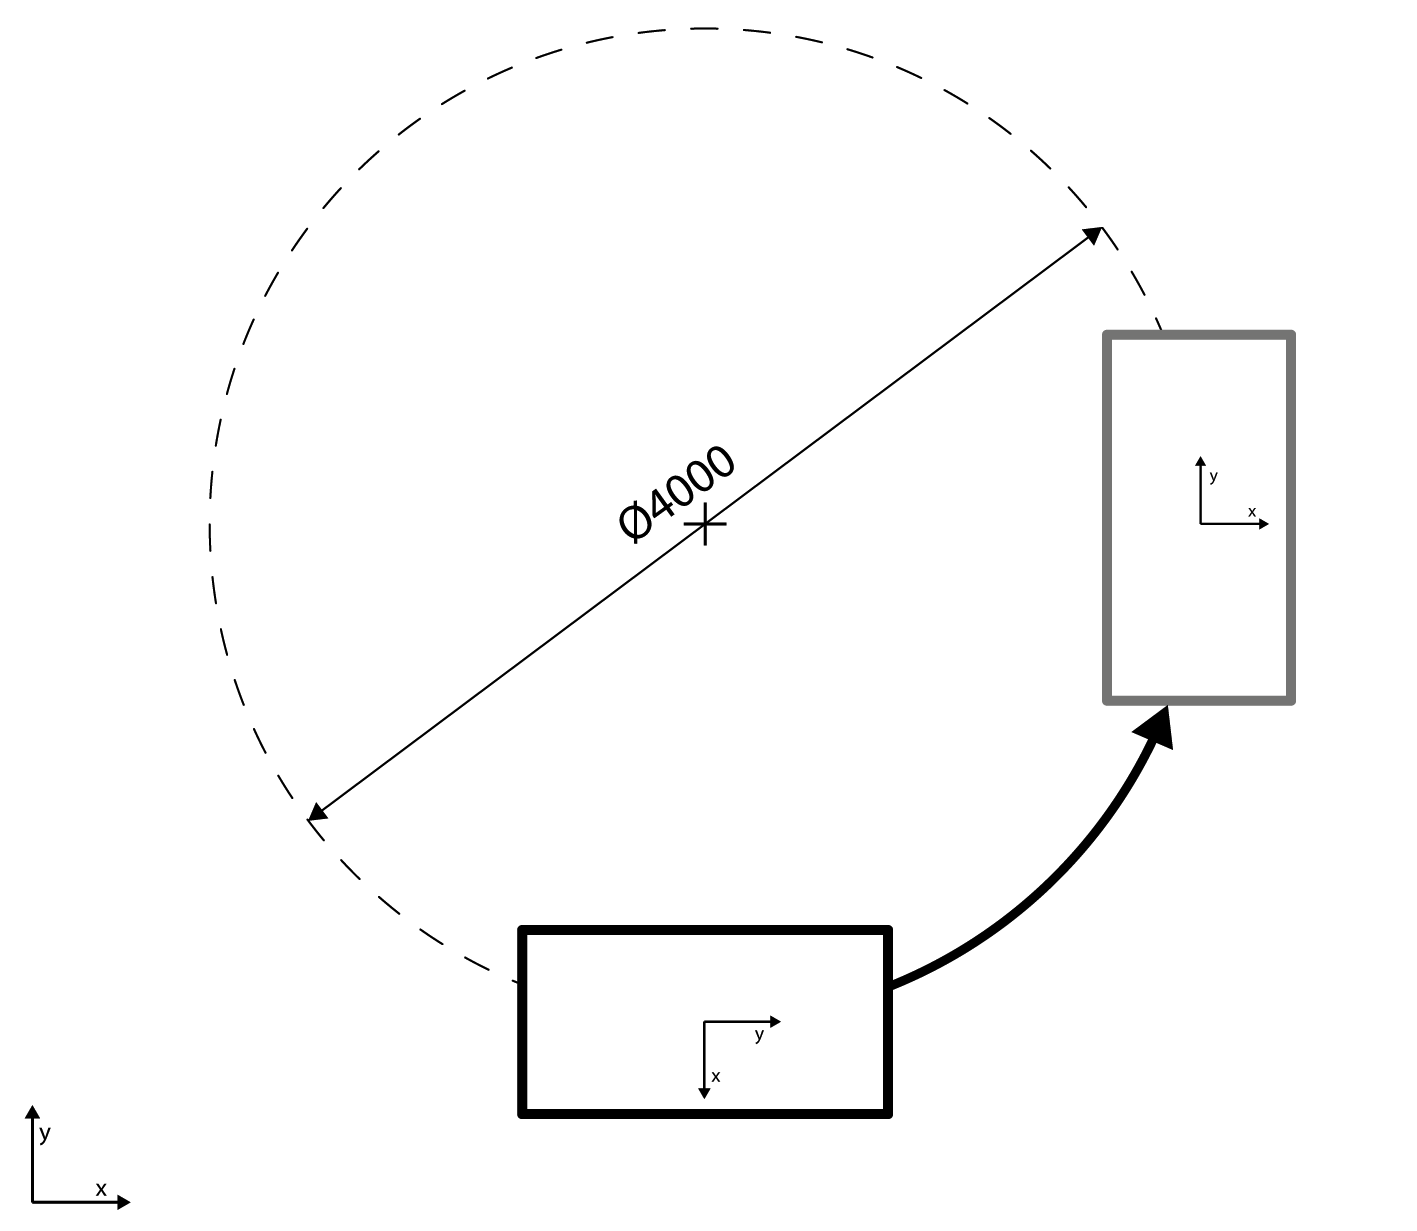
\includegraphics[width=.6\textwidth]{Viertelkreis-vorwaerts}
    \caption{Kreisfahrt vorwärts}
\end{figure}
Der Mecanum-Roboter fährt einen normalen Viertelkreis. Das Koordinatensystem des Roboters dreht sich dabei während der Kreisfahrt mit.

\begin{figure}[H]
    \centering
    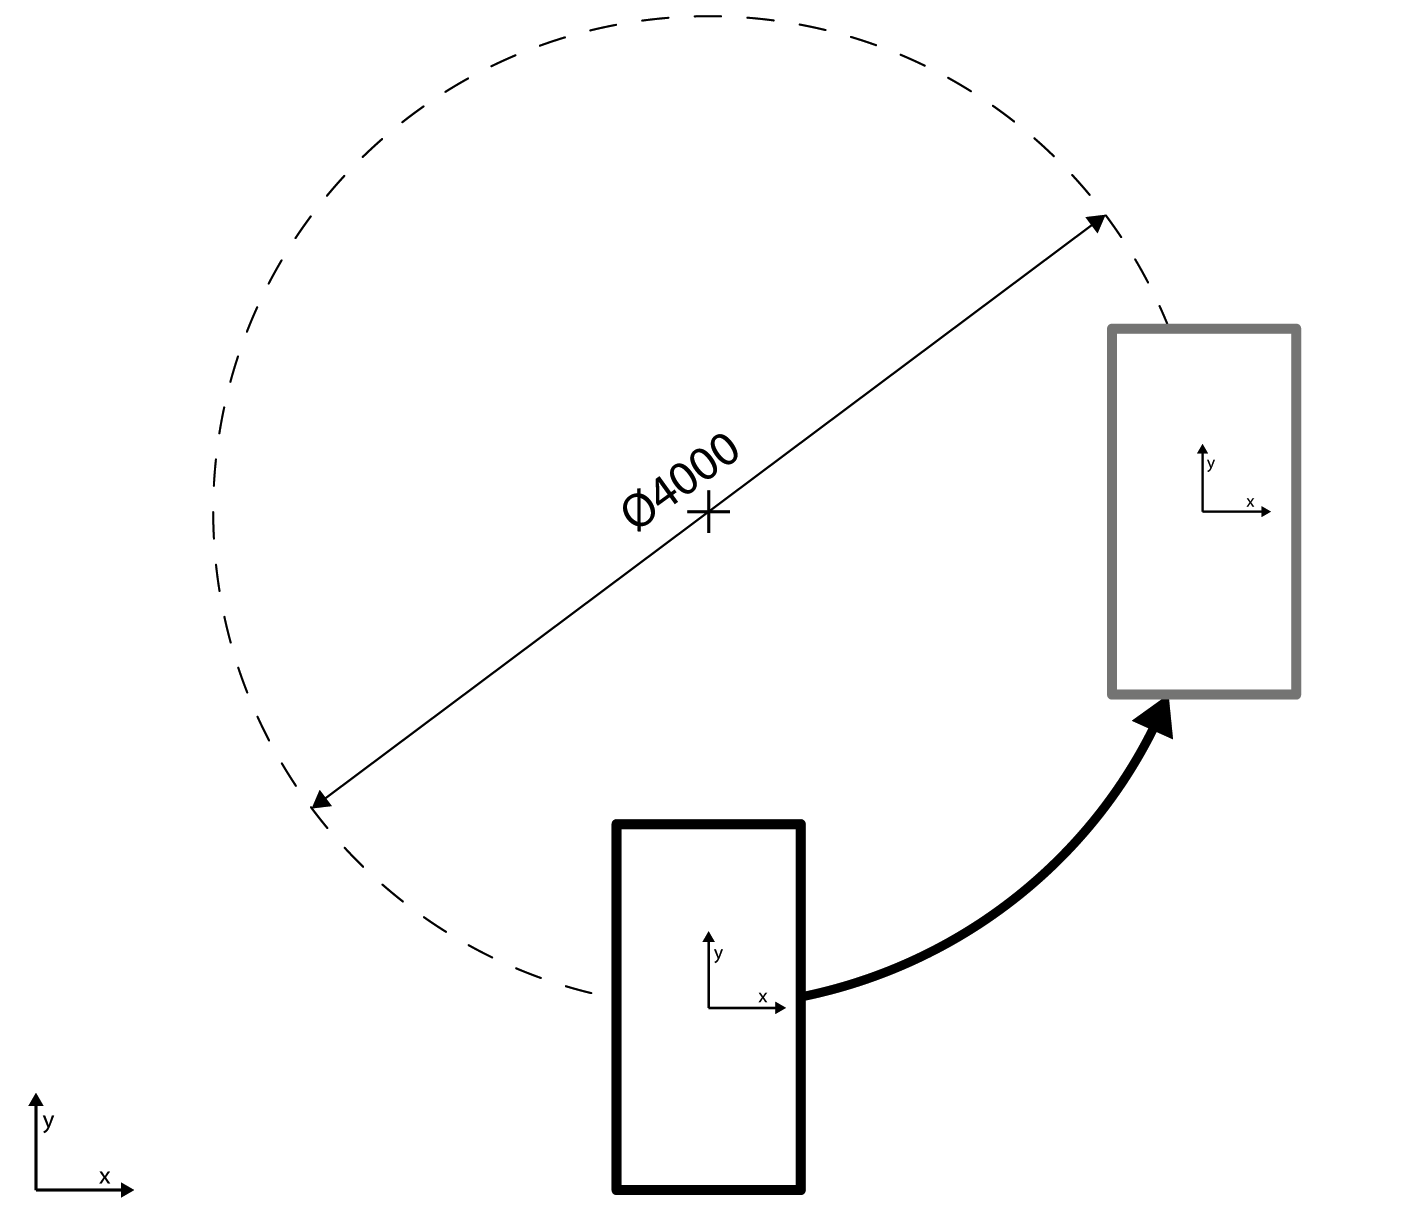
\includegraphics[width=.6\textwidth]{Viertelkreis-translatorisch}
    \caption{Translatorische Kreisfahrt}
\end{figure}
Die Koordinaten des Roboters liegen auf den Raumkoordinaten. Die parallele Ausrichtung bleibt während der Kreisfahrt bestehen.

\begin{figure}[H]
    \centering
    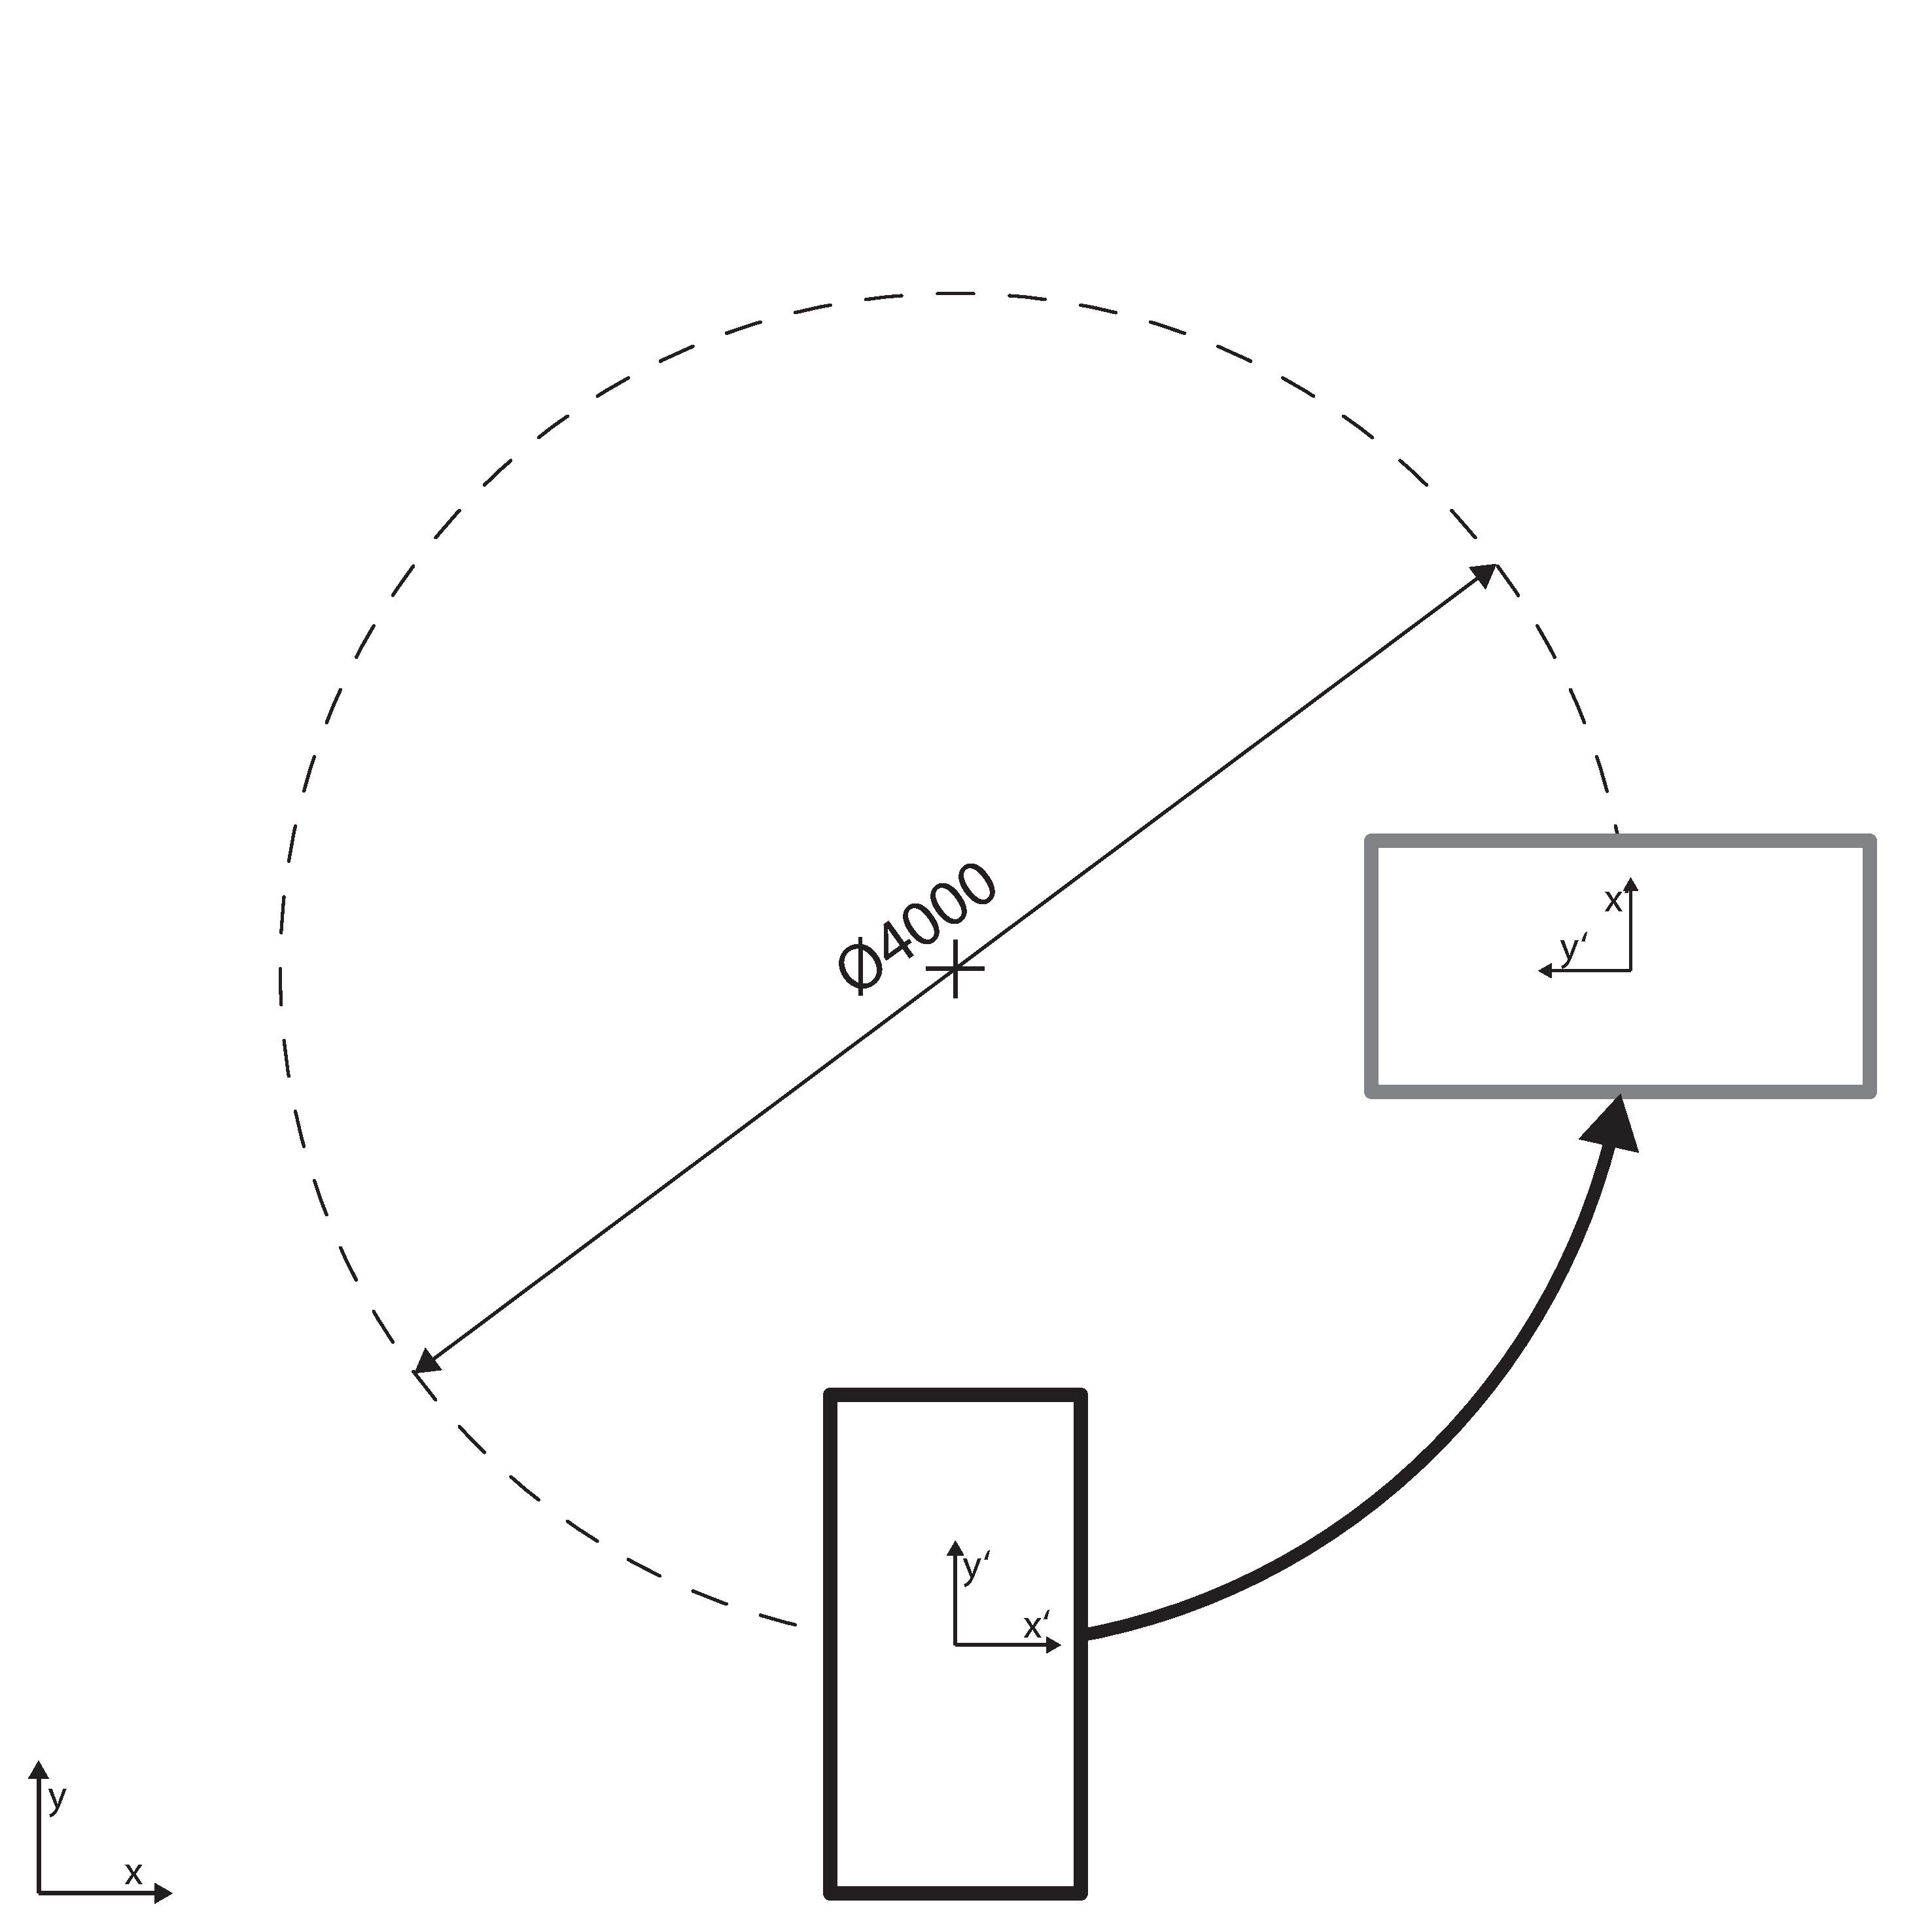
\includegraphics[width=.6\textwidth]{Viertelkreis-seitwaerts}
    \caption{Kreisfahrt seitlich}
\end{figure}
Das Koordinatensystem des Roboters ist um $90^\circ$ zum Raumkoodinatensystem gedreht. Bei der Kreisfahrt dreht sich der Roboter seitlich mit.


\section{Mathematik zur Kinematik / Dynamik}
Dieses Kapitel beschreibt die Mathematik hinter der Kinematik und Dynamik -- Bewegung unter Einwirkung von Kräften -- des Mecanum-Roboters. Jede Bewegung setzt sich aus einer translatorischen und einer rotatorischen Bewegung zusammen. So ist das auch das Kapitel gegliedert.

\subsection{Translation}
Vereinfacht kann die translatorische Bewegung des Mecanum-Roboters durch die Drehrichtung und Drehgeschwindigkeit der Mecanum-Räder beschrieben werden. Abhängig von den unterschiedlichen Kombination fährt der Roboter entlang des Vektors für die Gesamtbewegung.
\begin{figure}[H]
    \centering
    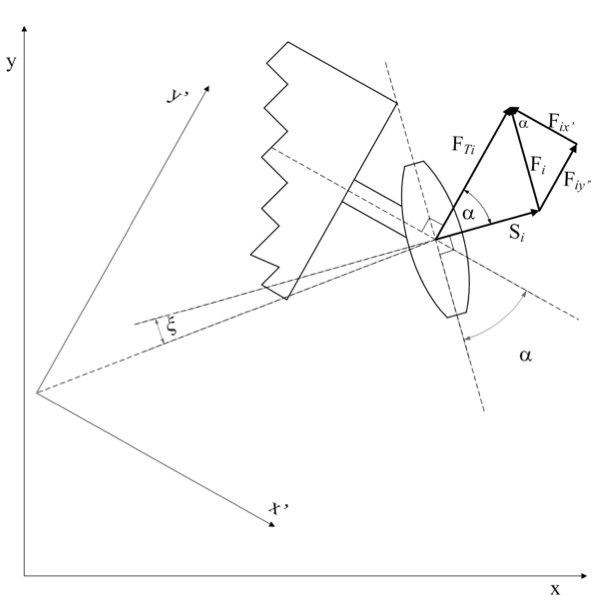
\includegraphics[width=.6\textwidth]{Kraefte-am-Rad}
    \caption{Kräftegleichgewicht an einem Mecanum-Rad.}
\end{figure}

Die Leistung einer vektoriellen Kraft berechnet sich nach:
$$ P_F = F_T \cdot v_F $$

Wirken Kraft und Geschwindigkeit entlang einer Koordinatenachse, haben beide Vektoren die gleiche Komponente ungleich null und ihr Skalarprodukt kann vereinfacht als Produkt der skalaren Größen betrachtet werden.

Die Kraftvektor in $x$- und $y$-Richtung setzt sich zusammen als die Summe der einzelnen $x$- und $y$-Vektoren der vier Räder:
\begin{align*}
    \sum_{i=1}^4 F_{iy} &= \sum_{i=1}^4 F_i \sin \alpha                 \\
    &= \sum_{i=1}^4 SIG \cdot K_i F_{Ti} \sin^2 \alpha                  \\
    &= \sum_{i=1}^4 SIG \cdot \frac{1}{2} K_i F_{Ti}                    \\
    \sum_{i=1}^4 F_{ix} &= \sum_{i=1}^4 F_i \cos \alpha                 \\
    &= \sum_{i=1}^4 (-1)^i SIG \cdot K_i F_{Ti} \sin \alpha \cos \alpha \\
    &= \sum_{i=1}^4 (-1)^i SIG \cdot \frac{1}{2} K_i F_{Ti}             \\
\end{align*}

SIG steht als Vorzeichenkonventionen für die Drehrichtung der Räder. Diese werden in der Steuerung direkt implementiert und werden daher bei den folgenden Rechnungen nicht weiter betrachtet.

Der Winkel $ \alpha $ liegt zwischen den Drehachsen der Rollen und der Räder ($\alpha = 45^\circ$).
Für eine translatorisch Bewegung müssen sich jeweils die diagonalen Räder (1, 3 und 2, 4) mit derselben Geschwindigkeit drehen. Entsprechen müssen ihre Kraftvektoren $F_{T1, 3} / F_{T2, 4}$ gleich groß sein.
Durch Auflösen der Summenzeichen erhält man ein Gleichungssystem:
\begin{align*}
    F_x &= - K_i F_{T1, 3} + K_i F_{T2, 4} \\
    F_y &= K_i F_{T1, 3}   + K_i F_{T2, 4}
\end{align*}

Nach Umstellen erhält man $F_{T1, 3}$ und $F_{T2, 4}$ und kann somit auch direkt die Geschwindigkeiten berechnen:
\begin{align*}
    F_{T1, 3} &= \frac{F_y + F_x}{K_i} &\Rightarrow v_{T1, 3} &= \frac{v_y + v_x}{K_i} \\
    F_{T2, 4} &= \frac{F_y - F_x}{K_i} &\Rightarrow v_{T2, 4} &= \frac{v_y - v_x}{K_i} \\
\end{align*}

Der Faktor $K_i$ setzt sich aus unterschiedlichen Faktoren zusammen, welche die durch das Motormoment erzeugten treibenden Kräfte beeinflussen und wird für den Boden der Werkstatt empirisch ermittelt.


\subsection{Rotation}
Die Rotation des Mecanum-Roboters um sein Zentrum kann durch die Drehrichtung der Räder bei gleicher Geschwindigkeit beschrieben werden.
Für eine Drehung im Uhrzeigersinn drehen Rad 1 und 2 rückwärts, Rad 3 und 4 vorwärts. Für eine Drehung gegen den Uhrzeigersinn entsprechend umgekehrt.
\begin{align*}
    v_{ref} &= K_i \cdot r \cdot \omega \\
    v_1 = v_4 &= - v_{ref}              \\
    v_2 = v_3 &= + v_{ref}
\end{align*}


\section{Koordinatentransformation}
Dieses Kapitel befasst sich mit der Koordinatentransformation vom ortsfesten Bezugskoordinatensystem zum Koordinatensystem des Mecanum-Roboters. \\
Die translatorische Verschiebung wird durch den Vektor $\underline T$ beschrieben.
\begin{align*}
\underline T =
\begin{bmatrix}
x_{T}\\
y_{T}\\
0
\end{bmatrix}
\end{align*}
Rotationsmatrix $\underline R$ um den Gierwinkel $\Psi$.
\begin{align*}
 \underline R_{\Psi} =
\begin{bmatrix}
  \cos{\Psi} & -\sin{\Psi} & 0\\
  \sin{\Psi} & \cos{\Psi} & 0\\
  0 & 0 & 1
\end{bmatrix}
\end{align*}
Positionsvektor des Roboter $\underline P$.
\begin{align*}
\underline P = \underline R_{\Psi} \cdot \underline T =
\begin{bmatrix}
  \cos{\Psi} & -\sin{\Psi} & 0\\
  \sin{\Psi} & \cos{\Psi} & 0\\
  0 & 0 & 1
\end{bmatrix}\cdot
\begin{bmatrix}
x_{T}\\
y_{T}\\
0
\end{bmatrix}=
\begin{bmatrix}
x_{T} \cdot \cos{\Psi}-y_{T} \cdot \sin{\Psi}\\
x_{T} \cdot \sin{\Psi}+y_{T}  \cdot \cos{\Psi}\\
0
\end{bmatrix}
\end{align*}
Als Ergänzung wird die Transformation bis zum Koordinatenursprung des montierten Roboterarms weitergeführt.
\begin{align*}
\underline T_{A} + \underline P =
\begin{bmatrix}
x_{A} + x_{T} \cdot \cos{\Psi}-y_{T} \cdot \sin{\Psi}\\
y_{A} + x_{T} \cdot \sin{\Psi}+y_{T}  \cdot \cos{\Psi}\\
z_{A}
\end{bmatrix}
\end{align*}


\section{Programmierung}
Der Roboter wird von einem Arduino Uno gesteuert, daher erfolgt die Programmierung in $C$. Das CAN-BUS Shield von SparkFun wird auf den Arduino aufgesteckt und ermöglicht die Kommunikation mit  den Schrittmotortreibern STMCI47 der Firma Nanotec.
Für die Umsetzung einer Kreisfahrt gibt es zwei Möglichkeiten:

\begin{enumerate}
\item \emph{Explizit, iterativ:} \\
Dem Roboter wird in einem festgelegten Takt mit den neuen Sollgeschwindigkeiten für die Räder gespeist. Die Sollgeschwindigkeiten können zur Laufzeit berechnet werden oder aus einer Lookup-Tabelle stammen.

Ein zu langsam eingestellter Takt führt zu polygonalen Fahrverläufen, die den Sollkreis lediglich annähern. Dementsprechend ist diese Methode auch gegenüber Taktänderungen sehr anfällig, welche beispielsweise auftreten, wenn andere Prozesse im Mikrocontroller zu viel Rechenzeit benötigen.

\item \emph{Implizit, funktionell:} \\
Die Soll-Radgeschwindigkeiten werden als Funktion abhängig von der Zeit seit Beginn der Kreisfahrt definiert. Sie können zu jedem beliebigen Zeitpunkt abgefragt werden. Das erlaubt dem Mikrocontroller seine Rechenzeit frei einzuteilen und resultiert in ruckfreien, flüssigen Bewegungsabläufen.
\end{enumerate}

Wegen dieser Vorteile wird die implizite Definition der Fahrbewegung implementiert.


\section{Schlussteil}
\subsection{Diskussion der Ergebnisse}

\subsection{Schwierigkeiten}
Bei der Umsetzung der Kreisfahren treten zahlreiche Schwierigkeiten auf, auf die über die Programmierung kein Einfluss zu nehmen ist.
\begin{compactitem}
    \item Untergrund uneben / Unebenheiten
    \item keine perfekt planaren Fläche
    \item Schmutz ändert Reibkoeffizient
    \item Motorenleistung zu schwach, verlieren Schritte
    \item Räder verhaken im Riementrieb
    \item Lagerung der Rollen auf den Rädern mangelhaft
    \item Befestigung und Lagerung der Rollen mangelhaft
\end{compactitem}

\end{document}
